\chapter{Project Planning and Management}
\section{The Triple Constraint Governance Model}
Developing a scheduling platform is a practical test case for applying the same project management principles that the software itself implements. To keep engineering effort focused and avoid uncontrolled feature growth, planning followed the classical \textbf{Triple Constraint Model} (the Project Management Triangle), shown in the figure below. In this framework, \textbf{Scope}, \textbf{Time}, and \textbf{Budget} act as coupled constraints that directly govern overall deliverable \textbf{Quality}: whenever one side is held fixed, the others must be balanced carefully so reliability does not degrade.

\begin{figure}[H]
    \centering
    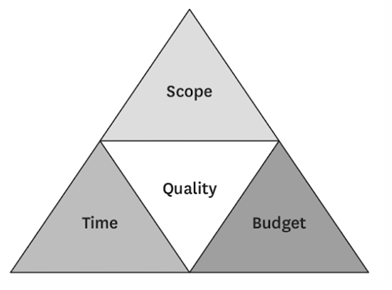
\includegraphics[width=0.38\textwidth]{images/Triple_Constraint.png}
    \vspace{-10pt}
\end{figure}

\vspace{-8pt}
\begin{itemize}[itemsep=1pt,topsep=0pt,parsep=0pt,partopsep=0pt]
    \item \textbf{Project Scope}: Scope was defined at the outset through a structured requirements review bounded around the six scheduling processes of PMBOK\textsuperscript{\textregistered} Chapter 6. Every proposed feature was checked against that core lifecycle, resulting in a containerized web architecture, schema-validated MongoDB storage, deterministic CPM/PERT/EVM engines, a 14-point DCMA audit, contributor time-tracking and controller review workflows, and \textit{Google Gemini Flash} NLP helpers. 
    \item \textbf{Budget}: Financial expenditure was fixed at \textbf{virtually zero (€0)}. Working without paid SaaS licenses or commercial enterprise software required relying entirely on open-source tooling (FastAPI, MongoDB Community Edition, Docker Compose, Vanilla JavaScript, \texttt{vis-network}, and \texttt{Chart.js}) together with free-tier Gemini Flash API quotas, trading capital spending for deliberate system design.
    \item \textbf{Time}: Execution spanned a seven-week, 53-day calendar window from September 21 to November 13, divided across architecture design, database setup, algorithmic implementation, UI refactoring, integration testing, documentation, and final vendor analysis. 
    \item \textbf{Quality}: Holding cost at zero and keeping scope sharply defined focused the entire seven-week time budget on internal craftsmanship and verification. This discipline made room for essential mid-project corrections, replacing a sluggish Streamlit prototype with JavaScript modules and realigning the WBS structure with PMBOK's 100\% rule, alongside strict MongoDB \texttt{\$jsonSchema} rules, in-memory LRU caching, and edge-case validation across schedules and APIs. 
\end{itemize}

\vspace{2mm}

In short, fixing the budget at €0 and drawing a clear boundary around schedule management allowed available time to go into iterative refactoring, mathematical verification, and testing whenever setbacks arose, turning tight constraints into higher final software quality.

\newpage

\section{Chronological Development Schedule and Execution}
Development progressed iteratively across the 53-day window, absorbing planned rest days, a multi-day interruption in late September, and several technical course corrections along the way: replacing an early Streamlit prototype with plain HTML/CSS/JavaScript (despite its faster development process, Streamlit's frontend proved unsatisfactory), re-aligning the WBS model with PMBOK's 100\% rule (initially I didn't quite understand how a WBS works), adding the 14-point DCMA audit, and recovering from local Git repository corruption (I had issues with Git and a corrupted commit). The table below records the full chronological milestone log.

\begin{table}[H]
\centering
\scriptsize
\renewcommand{\arraystretch}{0.90}
\caption*{Chronological Development Schedule and Milestone Execution Ledger (Sep 21 -- Nov 13).}
\begin{tabularx}{\textwidth}{l p{3.7cm} X}
\toprule
\textbf{Date / Period} & \textbf{Milestone / Domain} & \textbf{Key Deliverables \& Engineering Activities} \\
\midrule
Sep 21--24 & Ideation \& System Design & Requirements analysis, Database and Backend design, Frontend draft, PMBOK 6 mapping. \\
Sep 25--29 & Unforeseen Events (\textit{Force Majeure}) & Work paused due to external circumstances. \\
Sep 30 & DB Schema \& Docker Setup & MongoDB \texttt{\$jsonSchema} specifications, multi-container \texttt{docker-compose} topology. \\
Oct 1--3 & Authentication \& DB Seeding & Salted Bcrypt hashing, session tokens, Extended JSON/BSON data seeding. \\
Oct 4 & Scheduled Rest & Time off. \\
Oct 5--8 & UI Prototype \& Architectural Migration & Streamlit prototype discarded and migrated to Vanilla JS/HTML5/CSS. \\
Oct 9 & PM Workspace Architecture & Component modularization, unified navigation shell, responsive UI layout. \\
Oct 10 & Plan Schedule Management (6.1) & Process 6.1 dashboard, project charter configuration, working calendar setup. \\
Oct 11 & Scheduled Rest & Time off. \\
Oct 12 & Project Creation Page & Two-Stage Creation Process, Single vs. Multi-Team \& Open vs. Approval governance. \\
Oct 13 & Define Activities Dashboard (6.2) & Process 6.2 dashboard, Work Package decomposition, Vis-Network WBS tree. \\
Oct 14 & Activity Sequencing Inception (6.3) & PDM graph data structures, node models, dependency link abstractions. \\
Oct 15 & WBS Review \& Concept Realignment & Conceptual refactoring aligning activities with terminal WBS packages (PMBOK 100\% rule). \\
Oct 16--17 & Sequencing Dashboard (6.3) & Interactive PDM canvas, FS/SS/FF/SF dependencies, lead/lag adjustment, bug fixes. \\
Oct 18 & Scheduled Rest & Time off. \\
Oct 19--22 & Duration Estimation \& PERT (6.4) & DFS recursion cycle detection, Three-Point Beta math, target probability simulator. \\
Oct 23 & Schedule Dashboard (6.5) & CPM forward/backward passes, Total/Free Float, AON/AOA graphs, Gantt chart. \\
Oct 24 & Schedule Control Dashboard (6.6) & 4-tier execution states, Earned Value KPIs, S-Curve Banana Envelope tracking. \\
Oct 25 & Scheduled Rest & Time off. \\
Oct 26 & Testing \& Bug Fixes & Edge-case mathematical verification, zero-float validation, cache invalidation. \\
Oct 27 & Automated DCMA 14-Point Diagnostic & Defense-grade schedule health audit engine evaluating all 14 DCMA standards. \\
Oct 28 & Team Member Workspace & Contributor workspace, assigned operational agenda, execution Kanban board. \\
Oct 29 & Notification \& Subscription System & Multi-recipient notifications, join request approval, Controller review alerts. \\
Oct 30 & Gemini AI \& NLP Engine Integration & Text-to-WBS generation, PERT duration estimation, AI dependency extraction. \\
Oct 31 -- Nov 1 & Scheduled Rest & Time off (All Saints / All Souls break). \\
Nov 2 & Testing \& Bug Fixes & AI prompt hardening, JSON schema parsing validation, edge-case testing. \\
Nov 3--4 & Trello-Style Stopwatch Timers & Live activity timer widget, server-side duration logging, project time log history. \\
Nov 5 & NLP Engine Bug Fixes & Gemini model fallback hardening, external API rate limit resilience. \\
Nov 6 & Git Repository Recovery & Diagnosis and resolution of local Git file corruption. \\
Nov 7 & Final Testing \& Quality Assurance & End-to-end regression testing, UI polish, cross-browser responsiveness validation. \\
Nov 9 & Project Completion & Final release verification, documentation readiness, and project sign-off. \\
Nov 10--11 & Documentation & Project documentation has been prepared. \\
Nov 12--13 & Vendor Analysis & The project's Vendor Analysis has been prepared. \\
\bottomrule
\end{tabularx}
\end{table}
